\documentclass[../main.tex]{subfiles}
\graphicspath{{\subfix{../images/}}}
\begin{document}

O robô quadrúpede é um sistema robótico móvel que se locomove com a ajuda de pernas. Quando comparado a robôs terrestres que utilizam outros meios de locomoção --- como rodas ou esteiras ---, ele apresenta diversas particularidades que lhes confere muitas vantagens quanto à mobilidade, robustez a diferentes terrenos e superação de obstáculos \cite{Biswal2021}. Robôs com rodas e esteiras conseguem navegar pelo espaço, desde que haja um caminho contínuo entre os pontos de origem e de destino. Robôs com pernas, por outro lado, são capazes de escolher os melhores pontos no terreno para apoiar suas patas, o que permite uma navegação em caminhos discretos (com obstáculos de grande inclinação e variação de altura) \cite{Yao2021}. Essa capacidade de se adaptar a terrenos desnivelados favorece sua aplicação em diversos setores: industriais, militares, missões de inspeção e de resgate. Por outro lado, esse tipo de robô apresenta menor estabilidade de locomoção e, por consequência, maior complexidade de controle.

Robôs com pernas também apresentam diversas diferenças entre si, majoritariamente ligadas à quantidade de pernas que possuem. A quantidade de pernas de um robô está diretamente relacionada a sua estabilidade, capacidade de locomoção e eficiência. Os bípedes possuem baixa estabilidade, visto que se apoiam em apenas uma perna para poderem andar. Aqueles com múltiplas pernas (mais de quatro) possuem maior estabilidade, visto que conseguem manter pelo menos três pontos de apoio no solo enquanto realizam um passo. No entanto, cada perna representa um conjunto adicional de juntas e atuadores, diminuindo a eficiência do sistema como um todo. Os quadrúpedes conseguem unir vantagens desses dois tipos ao apresentar um balanço entre estabilidade e eficiência. Eles possuem uma estabilidade passiva quando estáticos, pois se apoiam em quatro pontos. Além disso, também são capazes de navegar de forma estável em baixas velocidades, movendo uma perna por vez enquanto as outras três permanecem no solo. Isso elimina a redundância presente nos robôs com múltiplas pernas, aumentando sua eficiência \cite{Yao2021}.

\subsection{Estrutura e design}
Pelo fato de robôs quadrúpedes terem se tornado um grande foco de pesquisa nos últimos anos, diferentes \textit{designs} já foram pesquisados. Esses \textit{designs} se diferenciam em aspectos como estrutura, configuração de pernas e o número de graus de liberdade (GDL) por perna.

Um dos tipos de estrutura que existem é a de tipo mamífero. A estrutura tipo mamífero tem esse nome devido a sua semelhança com a postura de quadrúpedes como cachorros e cavalos. Kitano \textit{et al.}, em \cite{Kitano2016}, analisa dois tipos diferentes de estruturas de robôs quadrúpedes: a do tipo mamífero (figura \ref{fig:robots_structures_b}) e a do tipo \textit{sprawling} (figura \ref{fig:robots_structures_c}). Segundo sua análise, a primeira permite alcançar maiores velocidades por possuir duas juntas no plano sagital. Além disso, ela também é mais eficiente, pois os atuadores requerem menos torque para sustentar o robô: sua estrutura mais compacta diminui o braço de alavanca sobre o qual a força peso do robô atua. Essa estrutura também favorece a navegação em ambientes estreitos, onde um robô do tipo \textit{sprawling}, por exemplo, teria dificuldades de acessar.

\begin{figure}[h]
  \centering
  \caption{Exemplos de robôs com estruturas do tipo mamífero e \textit{sprawling}.}
  % \begin{subfigure}[t]{0.32\textwidth}
  %   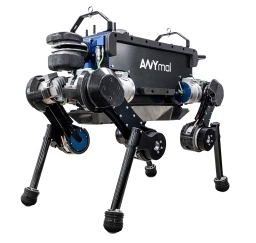
\includegraphics[width=1.0\textwidth]{Anymal.png}
  %   \caption{ANYmal.}
  %   \label{fig:robots_structures_a}
  % \end{subfigure}
  \begin{subfigure}[t]{0.23\textwidth}
    \centering
    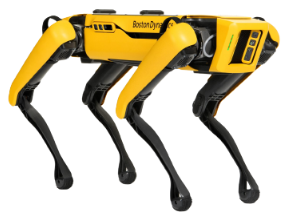
\includegraphics[width=0.9\textwidth]{Spot.png}
    \caption{Spot.}
    \label{fig:robots_structures_b}
  \end{subfigure}
  \begin{subfigure}[t]{0.23\textwidth}
    \centering
    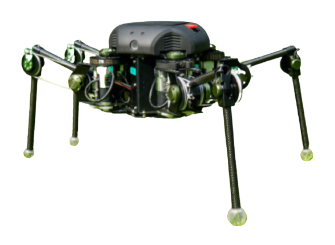
\includegraphics[width=1.0\textwidth]{Titan.png}
    \caption{TITAN-XIII.}
    \label{fig:robots_structures_c}
  \end{subfigure}
  \vfill
  Fonte: Adaptado de  \cite{Kitano2016} e \cite{SpotImg1}.
  \label{fig:robots_structures}
\end{figure}
\vspace{-1.5\parskip}

Os robôs quadrúpedes que utilizam essa estrutura também se diferenciam quanto à configuração das pernas. As duas configurações mais utilizadas podem ser vistas na figura \ref{fig:joint_configurations}. Robôs como o \textit{Spot}, \textit{MIT Cheetah} e \textit{Stanford Pupper} utilizam a configuração \textit{full-elbow}, enquanto outros como o \textit{ANYmal}, \textit{StarlETH} e \textit{BigDog} adotam a configuração \textit{elbow-knee}. Yao \textit{et al.}, em \cite{Yao2021}, acreditam que a configuração \textit{elbow-knee} possibilita maior estabilidade, mas as características de movimento da configuração \textit{full-elbow} podem ser superiores.

\begin{figure}[h]
  \centering
  \caption{Tipos de configuração de pernas para robôs com estrutura tipo mamífero.}
  \begin{subfigure}[t]{0.24\textwidth}
    \centering
    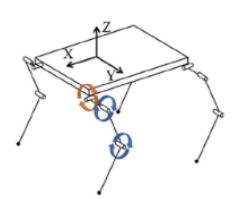
\includegraphics[width=1.0\textwidth]{full_elbow.png}
    \caption{\textit{full-elbow}.}
    \label{fig:joint_configurations_a}
  \end{subfigure}
  % \begin{subfigure}[t]{0.24\textwidth}
  %   \centering
  %   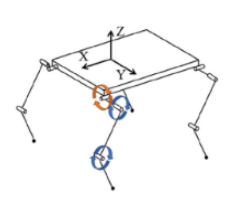
\includegraphics[width=1.0\textwidth]{full_knee.png}
  %   \caption{\textit{full-knee}.}
  %   \label{fig:joint_configurations_b}
  % \end{subfigure}
  % \begin{subfigure}[t]{0.24\textwidth}
  %   \centering
  %   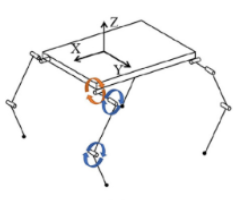
\includegraphics[width=1.0\textwidth]{knee_elbow.png}
  %   \caption{\textit{knee-elbow}.}
  %   \label{fig:joint_configurations_c}
  % \end{subfigure}
  \begin{subfigure}[t]{0.24\textwidth}
    \centering
    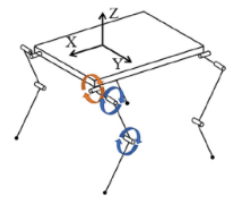
\includegraphics[width=1.0\textwidth]{elbow_knee.png}
    \caption{\textit{elbow-knee}.}
    \label{fig:joint_configurations_d}
  \end{subfigure}

  Fonte: Adaptado de \cite{Yao2021}.
  \label{fig:joint_configurations}
\end{figure}

O número de juntas nas pernas, que coincide com a quantidade de GDL do robô, também é um dos aspectos estudados sobre os quadrúpedes. A maioria apresenta 3 GDL por perna, o que é suficiente para que o robô consiga mover suas patas em três dimensões e realize diversos tipos de marchas. A fim de simplificar a estrutura e consequentemente o controle, alguns robôs utilizam apenas 2 GDL por perna, eliminando a junta no corpo que movimenta a perna no plano frontal. Outros robôs buscam performances mais semelhantes ao andar de animais reais, o que demanda maior flexibilidade de movimento, justificando o acréscimo de uma quarta junta. No entanto, como já mencionado, esse acréscimo aumenta a complexidade do controle e prejudica a eficiência. Essa perda de eficiência se dá porque a maior quantidade de atuadores resulta em um maior consumo de energia e também mais massa.

A massa do robô quadrúpede deve ser a menor possível. Quanto mais leve for o sistema, menos torque será demandado dos motores e maior sua eficiência. Além disso, a distribuição de massa do robô também é um aspecto muito importante. A massa deve ser localizada majoritariamente no corpo, enquanto as pernas devem possuir baixa inércia. Isso permite que elas se movam rapidamente sem alterar, de forma significativa, o centro de gravidade do robô, o que aumenta a estabilidade e requer menos complexidade de controle. Possuir baixa inércia significa possuir baixa massa. Por outro lado, as pernas devem ser resistentes o suficiente para suportar o peso do robô, além dos distúrbios causados pelo impacto das patas com o chão, o que pode demandar um aumento de massa nas pernas. Portanto, um equilíbrio entre massa e resistência deve ser buscado ao mesmo tempo em que deve-se buscar diminuir a massa total do sistema \cite{Zhong2019}.

\subsection{Movimentação por marchas}
Robôs quadrúpedes se movimentam conforme uma sequência de movimentos coordenados de suas pernas que compõem uma marcha. Uma marcha é definida pelo tempo e local de colocação e levantamento de cada pata, coordenado com o movimento do corpo em seus seis graus de liberdade, para mover o corpo de um lugar para outro  \cite{Song1989}.

A marcha é um aspecto fundamental para garantir que um robô com pernas caminhe de forma eficiente e estável, especialmente em terrenos irregulares \cite{X.129}. Para isso, é necessário levar em consideração suas etapas e, consequentemente, seu tipo.

Marchas são divididas em duas etapas: \textit{stance} e \textit{swing}. Durante a fase \textit{stance}, as pernas estão no solo e impulsionam o robô para frente. Na etapa de \textit{swing}, as pernas são erguidas para deslocar a pata até o próximo ponto de apoio. É importante ressaltar que as fases de \textit{stance} e \textit{swing} não ocorrem em todas as pernas simultaneamente. A depender do tipo de marcha, algumas pernas podem estar em \textit{swing} enquanto outras estarão em \textit{stance}.

O \textit{trot} é um tipo de marcha muito utilizado por robôs quadrúpedes, devido a sua simplicidade e eficiência. Este tipo de marcha é periódico e simétrico. Marchas periódicas são caracterizadas pela repetição contínua dos mesmos movimentos nos mesmos instantes, dentro de um ciclo de locomoção \cite{de2006quadrupedal}. Já a simetria é uma característica de marchas que movimentam um par de pernas em conjunto, saindo e voltando para o solo de forma sincronizada. No \textit{trot}, as pernas diagonais se movimentam em pares e quando um par está na etapa de \textit{swing}, o outro está na etapa de \textit{stance}. Outra característica da marcha \textit{trot} é que ela pode ser contínua ou descontínua. Uma marcha contínua mantém o corpo do robô em movimento constante, enquanto a descontínua submete o corpo a um movimento intermitente \cite{de2006quadrupedal}. Portanto, quando a marcha \textit{trot} é contínua, as pernas em \textit{stance}, além de sustentarem o robô, deslocam o corpo na direção do movimento, o que exige maior capacidade de controle. Em contrapartida, quando ela é descontínua, o corpo fica estático esperando as pernas em \textit{swing} terminarem seu movimento para, então, ser deslocado, tão logo as quatro pernas estejam no solo.

\subsection{Controle de locomoção}

Todo o controle de locomoção do robô é realizado pelo planejador de marchas. Ele é o responsável por enviar os comandos para que as pernas se movam para os locais desejados no momento esperado. Logo, o planejador irá apenas ditar o ponto no espaço no qual cada pata do robô deve estar, em relação a um eixo de referência, cabendo ao sistema de controle executar o movimento. A seguir, serão discutidos dois itens fundamentais do sistema de controle de um robô quadrúpede: o modelo cinemático e as estratégias de controle.

\subsubsection{Modelo cinemático}
O modelo cinemático de um robô quadrúpede descreve a relação entre a posição de uma pata em três dimensões com a rotação de cada junta da sua respectiva perna. Como todas as pernas do robô são iguais, pode-se formular as relações de apenas uma perna e replicá-la quatro vezes, acrescentando as devidas translações e rotações, para obter o modelo cinemático de todo o sistema.

O modelo cinemático pode ser usado para resolver dois problemas: a cinemática direta e a cinemática inversa. A cinemática direta fornece a posição de uma pata em $(x, y, z)$ em função dos ângulos das juntas, enquanto que a cinemática inversa fornece os ângulos das juntas correspondentes a uma posição da pata no espaço tridimensional. Esses dois problemas são complementares, sendo a saída de um a entrada do outro, e vice-versa. A partir da cinemática inversa, o robô consegue determinar quanto deve rotacionar seus atuadores para mover a pata a alguma distância nas direções $(x, y, z)$. Com a cinemática direta, é possível saber se a pata de fato chegou na posição em que ele deveria estar. Portanto, ambos são muito importantes para o controle de locomoção do robô.

\subsubsection{Estratégias de controle}
A locomoção de robôs quadrúpedes, em geral, segue uma sequência de passos. Raibert propõe em \cite{Raibert1986} um método de controle baseado em três etapas: controle de salto, controle de velocidade e controle de postura do corpo. Essa estratégia de controle foi utilizada para controlar robôs com uma, duas e quatro pernas (o motivo de se ter um controle de salto é que robôs com apenas uma perna só podem ser locomover saltando). Sua premissa básica era a de que apenas uma perna estaria em \textit{stance} ou em \textit{swing} por vez. A fim da satisfazer essa premissa para robôs com mais de duas pernas, foi proposto o conceito de pernas virtuais. Isto é, um conjunto de pernas deve realizar igual comportamento quando em \textit{swing} e \textit{stance} e as fases de \textit{swing} e \textit{stance} de cada conjunto devem ser alternadas. Esse conceito foi utilizado para embasar o uso de marchas simétricas e periódicas como o \textit{trot}.

Essa estratégia de controle em três etapas foi responsável por locomover robôs com pernas rígidas (apenas 2 GDL por perna, sendo uma junta rotativa e outra prismática) de maneira simples. No entanto, esses robôs apenas operavam no terreno plano e controlado do laboratório. A fim de possibilitar a operação de robôs com pernas em terrenos desnivelados e de difícil mobilidade, Raibert \textit{et al.} propôs um outro sistema de controle no seu trabalho sobre o \textit{BigDog} \cite{RAIBERT200810822}. O \textit{BigDog} é um robô quadrúpede com 4 GDL por perna movido por atuadores hidráulicos. Essa maior flexibilidade de movimentação das pernas permite controlar a locomoção do robô sem que este precise saltar, sendo possível, então, dividir o controle de locomoção em duas etapas principais: controle de \textit{stance} e controle de \textit{swing}. Como o nome sugere, o controlador de \textit{stance} é o responsável por controlar o comportamento das pernas na fase de \textit{stance}, enquanto o controlador de \textit{swing} é o responsável por controlar as pernas em \textit{swing}. Vale lembrar que durante a marcha, algumas pernas podem estar na etapa de \textit{swing} enquanto outras estão na etapa de \textit{stance}, o que significa que esses controladores ora assumem o comando de um par de pernas, ora de outro (essa troca não necessariamente se dá em pares, porém isso é válido para marchas simétricas como o \textit{trot}). Quem define o momento em que cada controlador assume o controle de uma determinada perna é o planejador de marchas.

O modo como cada perna se comporta durante as etapas de \textit{stance} e \textit{swing} pode variar em diversos aspectos, mas ainda é possível elencar semelhanças gerais. No início da etapa de \textit{swing}, calcula-se o local do próximo ponto de apoio das patas com base na velocidade desejada para o robô e uma trajetória de passo até esse ponto. Essa trajetória pode ter o formato de uma curva senoidal \cite{X.118}, triangular \cite{StanfordPupper}, de Bezier \cite{HackadayQuadruped}, cicloidal \cite{Shi2021} \cite{X.58}, entre outras. Uma consideração que pode ser feita a fim de simplificar o sistema de controle é de que a movimentação das pernas durante a fase de \textit{swing} não interfere no movimento do corpo do robô. Para que isto seja válido, é necessário controlar a força com que a pata toca o solo, a fim de diminuir os distúrbios causados no corpo do robô. A força de contato entre as patas e o solo é um ponto-chave para a estabilidade do quadrúpede \cite{X.118}. Nesse sentido, a trajetória cicloidal ganha destaque por conta de sua primeira derivada nula no momento em que se aproxima do seu ponto mínimo.

Já na fase de \textit{stance}, as pernas devem manter o robô em equilíbrio, além de deslocar o corpo na direção desejada de locomoção. Para isso, alguns robôs utilizam trajetórias para as patas com um formato pré-determinado, assim como na fase de \textit{swing}, não necessariamente repetindo o mesmo formato de curva \cite{X.118, X.58}. Além disso, controladores de equilíbrio também podem ser implementados nessa etapa. Esses controladores visam estabilizar os ângulos de \textit{pitch} e \textit{roll} do robô \cite{Shi2021, StanfordPupper, HackadayQuadruped, Notspot} ou até ainda outros graus de liberdade \cite{X.134, Chen2020140736, Zhang2016284}. Eles podem controlar diretamente a angulação do corpo do robô (com o auxílio de um sensor inercial) e/ou a força de contato com o solo em cada perna, por exemplo. No entanto, alguns trabalhos se baseiam apenas no controle individual de cada junta para manter o robô em equilíbrio, o que é uma abordagem mais simples, mas que pode falhar especialmente em terrenos irregulares.

\end{document}
